\documentclass[11pt,a4paper]{report}
\usepackage[margin=1in]{geometry}
\usepackage{amsmath,amssymb,amsfonts}
\usepackage{graphicx}
\usepackage{booktabs}
\usepackage{longtable}
\usepackage{array}
\usepackage{hyperref}
\usepackage{enumitem}
\usepackage{xcolor}
\usepackage{float}
\usepackage{caption}
\usepackage{subcaption}

\hypersetup{colorlinks=true,linkcolor=blue!60!black,citecolor=blue!60!black,urlcolor=blue!60!black}

\title{%
  \textbf{Experiments 1A--1C: Detailed Technical Report}\\[0.4em]
  \large Mathematical Gate, Discovery Atlas, and Adaptive Refinement\\
  \normalsize Query--Key Initialization Geometry Research Program
}
\author{Automated report from frozen artifacts in \texttt{code/exp1a/data/full}, \texttt{code/exp1b/data/full}, and \texttt{code/exp1c/data/full}}
\date{September 6, 2026}

\newcommand{\Hnorm}{H_{\mathrm{norm}}}
\newcommand{\dd}{\mathrm{d}}

\begin{document}
\maketitle
\tableofcontents
\clearpage

%=============================================================================
\chapter{Executive Summary}
%=============================================================================

This document records the confirmatory analysis for the first three stages of the initialization-atlas program:
\begin{itemize}[leftmargin=*]
  \item \textbf{Experiment 1A} (mathematical and implementation gate): \textbf{PASSED}. All $864$ Monte Carlo moment configurations and all auxiliary integration checks succeeded under preregistered tolerances.
  \item \textbf{Experiment 1B} (discovery atlas): \textbf{COMPLETE}. The full $1{,}717$-cell coefficient grid was measured at reference geometry $(d,m,n)=(64,16,64)$ across $879{,}104$ raw forward/backward records; bootstrap analysis produced $13{,}736$ stratified summaries.
  \item \textbf{Experiment 1C} (adaptive refinement + transfer): \textbf{MEASURED, PORTFOLIO NOT FROZEN}. $120$ surrogate-chosen cells $\times$ $2$ geometries $=240$ tasks, $122{,}880$ raw rows, $1{,}920$ stratified summaries. Held-out surrogate accuracy is high, but no coefficient point is \texttt{screened\_candidate} on every replicated stratum, so \texttt{candidate\_portfolio.json} remains unfrozen.
\end{itemize}

\textbf{Headline 1B findings} (all strata pooled, $N=13{,}736$ bootstrap-labeled summaries):
\begin{center}
\begin{tabular}{lrr}
\toprule
Label & Count & Fraction \\
\midrule
Diffuse & 5{,}362 & 39.0\% \\
Concentrated & 3{,}793 & 27.6\% \\
Screened candidate & 2{,}867 & 20.9\% \\
Boundary / uncertain & 1{,}241 & 9.0\% \\
Self-locked & 472 & 3.4\% \\
Gradient-starved & 1 & $<0.01$\% \\
\bottomrule
\end{tabular}
\end{center}

These labels are \textbf{descriptive} statements about initialization-time attention geometry. They are \emph{not} claims about downstream language-model quality until validated in Experiment~1D.

\textbf{Headline 1C findings} ($N=1{,}920$ adaptive/transfer summaries):
\begin{center}
\begin{tabular}{lrr}
\toprule
Label & Count & Fraction \\
\midrule
Diffuse & 793 & 41.3\% \\
Boundary / uncertain & 613 & 31.9\% \\
Screened candidate & 514 & 26.8\% \\
Concentrated / self-locked / gradient-starved & 0 & $0\%$ \\
\bottomrule
\end{tabular}
\end{center}
The adaptive sampler targeted uncertain and theory-disagreement cells, so concentrated/self-locked pathology is absent by design. Transfer majority-label agreement between $(64,16,64)$ and $(128,16,128)$ is only $30/120$ coefficient points.

%=============================================================================
\chapter{Scientific Context and Motivation}
%=============================================================================

\section{What problem is being studied?}

Transformer attention computes, for each query position $i$ and key position $j$,
\[
\ell_{ij} = \frac{1}{\sqrt{m}}\,(W_q x_i)^\top (W_k x_j),
\qquad
P_{ij} = \frac{\exp(\ell_{ij})}{\sum_{j'} \exp(\ell_{ij'})},
\]
where $W_q,W_k\in\mathbb{R}^{m\times d}$ are query and key projections and $x_i,x_j\in\mathbb{R}^d$ are token representations.

Standard initializers (e.g.\ Xavier/Kaiming on independent Gaussian weights) fix marginal variances but do not explicitly control the \textbf{joint geometry} of $(W_q,W_k)$. The research program introduces a \textbf{correlated Gaussian--orthogonal} family parameterized by $(s,\alpha,\beta,\gamma)$ (and angle $\phi$), derives \textbf{exact finite-width} expressions for logit moments, and then \textbf{maps} where different attention behaviors occur in coefficient space before testing trainability and real-model effects.

\section{Why staged experiments before training a large LM?}

\begin{enumerate}[leftmargin=*]
  \item \textbf{1A} answers: ``Is the theory implemented correctly?'' If not, every map is meaningless.
  \item \textbf{1B} answers: ``Where in $(s,\alpha,\phi)$ do diffuse, concentrated, self-locked, and screened behaviors occur at initialization?'' This is an empirical atlas, not a hand-drawn phase diagram.
  \item \textbf{1C} answers: ``Do uncertain/boundary cells remain screened under a fitted surrogate, extra samples, and a width/length transfer?'' A frozen portfolio is required before 1D.
\end{enumerate}

Failure of 1A would block all downstream confirmatory interpretation. \textbf{1A passed.} Therefore 1B--1C maps may be interpreted as proposal evidence for the discovery atlas (subject to the limitations in Chapter~\ref{ch:limitations}). The 1C freeze rule has \textbf{not} yet produced a training portfolio.

%=============================================================================
\chapter{Parameterization and Terminology Glossary}
%=============================================================================

\section{Coefficient tuple $(s,\alpha,\beta,\gamma)$}

Each admissible initialization is encoded by:
\begin{itemize}[leftmargin=*]
  \item $s>0$: \textbf{scale} controlling overall query/key energy. We report $\log_2 s$ on atlas plots.
  \item $\alpha\in[-1,1]$: \textbf{entrywise correlation} between flattened query and key coordinates within a head (target marginal correlation of $Q_{ab}$ and $K_{ab}$).
  \item $\beta,\gamma$: split between a \textbf{row-space orthogonal} component $B$ and an \textbf{independent Gaussian} component $C$ in the construction $W_q W_k^\top = s^2(AB^\top + C)$ with constraints ensuring valid covariance.
  \item $\phi\in[0,\pi/2]$: angle parameterizing $(\beta,\gamma)$ on the admissible circle at fixed $\alpha$.
\end{itemize}

At $\alpha=\pm 1$, $\phi$ is redundant (all angles collapse to the same point); the grid retains one endpoint representative per sign.

\section{Token geometry notation}

For tokens $x_i,x_j$ with Gram entries $v_i=\|x_i\|_2^2/d$, $v_j=\|x_j\|_2^2/d$, $c_{ij}=x_i^\top x_j/d$:
\begin{itemize}[leftmargin=*]
  \item \textbf{Predicted logit mean/variance}: closed-form $\mathbb{E}[\ell_{ij}]$ and $\mathrm{Var}(\ell_{ij})$ from Lemma~1 (verified in 1A).
  \item $\widehat\tau$: row-centered logit scale (empirical std.\ dev.\ of active logits in a row).
  \item $\widehat\Delta$: \textbf{diagonal gap}---mean diagonal logit minus mean off-diagonal logit on the active set.
\end{itemize}

\section{Attention-distribution metrics (1B)}

For each attention row $P_{i\cdot}$ over active keys $k_i>1$:
\begin{description}[style=nextline,leftmargin=2.2cm]
  \item[Normalized entropy $\Hnorm$]
    $H(P_{i\cdot})/\log k_i$. Equals $1$ for uniform attention; near $0$ for nearly one-hot rows.
  \item[Distance from uniform $d_{\mathrm{unif}}$]
    RMS $\|P_{i\cdot}-u_i\|_2$ where $u_i$ is uniform on the active support.
  \item[Maximum mass $\max_j P_{ij}$]
    Largest probability in the row (peakedness).
  \item[Self-mass $P_{ii}$]
    Diagonal attention probability (self-locking diagnostic).
  \item[Attention effective rank]
    $\mathrm{erank}(P)/n$ where $\mathrm{erank}(P)=\exp(-\sum_k \lambda_k\log\lambda_k)$ on singular values of the probability matrix.
  \item[Jacobian operator norm $\|J\|_2$]
    Spectral norm of softmax Jacobian $J(P_{i\cdot})=\mathrm{diag}(P_{i\cdot})-P_{i\cdot}P_{i\cdot}^\top$ (local sensitivity / gradient health).
  \item[Update-to-weight ratio]
    $\|\nabla W\|\cdot\eta/\|W\|$ from a single backward step on a synthetic one-batch MSE probe (not full LM training).
  \item[Kernel metrics]
    Singular values of $M=W_q^\top W_k$ (operator norm, effective rank, spectral concentration).
\end{description}

\section{Preregistered descriptive labels}

Labels are assigned from \textbf{95\% bootstrap confidence intervals} (2{,}000 seed-resampling draws per stratum in this run) with precedence:
\[
\text{self-locked} \succ \text{concentrated} \succ \text{diffuse} \succ \text{gradient-starved} \succ \text{screened candidate} \succ \text{boundary/uncertain}.
\]

\begin{description}[style=nextline,leftmargin=2.6cm]
  \item[Diffuse]
    Lower CI bound on median $\Hnorm \ge 0.95$ and upper CI bound on $d_{\mathrm{unif}}\le 0.10$.
  \item[Concentrated]
    Upper CI bound on median $\Hnorm\le 0.50$, \emph{or} lower CI bound on median $\max_j P_{ij}\ge 0.80$.
  \item[Self-locked]
    Lower CI bound on median self-mass $\ge 0.80$.
  \item[Gradient-starved]
    Upper CI bound on Jacobian or update-to-weight below pilot floors (see Section~\ref{sec:pilot-thresholds}).
  \item[Screened candidate]
    No pathology above confirmed; $\Hnorm$ between $0.60$ and $0.95$; attention effective rank above pilot floor.
  \item[Boundary / uncertain]
    Intervals cross thresholds (genuine measurement uncertainty).
\end{description}

\textbf{Important:} ``Screened candidate'' means ``passes forward pathology screens,'' not ``will train well.'' Trainability is Experiment~1D.

%=============================================================================
\chapter{Experiment 1A: Mathematical and Implementation Gate}
%=============================================================================

\section{Purpose}

1A is a \textbf{blocking quality-control stage}. It does not discover scientific novelty; it verifies that the codebase correctly implements:
\begin{itemize}[leftmargin=*]
  \item exact logit mean and variance formulas (Lemma~1);
  \item energy identities and entrywise variance targets;
  \item gradient/backprop identities (Proposition~4);
  \item common-bias cross-head statistic (Proposition~5);
  \item model integration (custom initializer, checkpoint survival, forward finiteness).
\end{itemize}

\section{Experimental design}

\subsection{Configuration grid}

\begin{itemize}[leftmargin=*]
  \item Widths $d\in\{32,64,128\}$.
  \item Head ratios $m/d\in\{1/8,1/4,1/2\}$.
  \item Token-pair correlations $c_{ij}\in\{-0.5,0,0.5,1.0\}$ (fixed synthetic pairs).
  \item $24$ coefficient points per geometry: four canonical corners plus $20$ interior $(\alpha,\phi)$ points.
\end{itemize}

Total moment configurations: $3\times 3\times 4\times 24 = 864$.

\subsection{Monte Carlo protocol}

For each configuration:
\begin{enumerate}[leftmargin=*]
  \item Draw $W_q,W_k$ from the admissible construction at the specified $(s,\alpha,\beta,\gamma)$.
  \item Compute empirical mean and variance of $\ell=(W_q x)^\top(W_k y)/\sqrt{m}$ over increasing draws (minimum $20{,}000$, up to $200{,}000$).
  \item Stop when $\mathrm{SE}(\widehat\mu)\le 0.01\,\sigma_{\mathrm{pred}}$ and $\mathrm{SE}(\widehat{\mathrm{Var}})\le 0.01\,\mathrm{Var}_{\mathrm{pred}}$.
  \item Record energies, orthogonality $\|AB^\top\|_F/(\|A\|_F\|B\|_F)$, entry variances, empirical entry correlation vs.\ $\alpha$.
\end{enumerate}

\subsection{Hypothesis tests}

For each configuration we form two-sided normal approximate $p$-values for mean and variance. Across all $864$ configurations ($1{,}728$ tests), \textbf{Holm--Bonferroni} correction controls family-wise error at $\alpha=0.01$. A configuration \textbf{passes} only if:
\begin{itemize}[leftmargin=*]
  \item neither corrected mean nor variance test is rejected;
  \item precision targets met;
  \item relative orthogonality $<10^{-6}$;
  \item component energies within $1\%$ of $s^2 m$ (and $B,C$ within $1\%$ of $m$);
  \item entry variances within $2\%$ of $s^2/d$;
  \item $|\widehat\rho_{\mathrm{entry}}-\alpha|\le 0.02$.
\end{itemize}

\subsection{Auxiliary checks (\texttt{checks.json})}

\begin{itemize}[leftmargin=*]
  \item \textbf{Gradient identity}: 20 random small configurations; analytic vs.\ finite-difference relative error $<10^{-5}$.
  \item \textbf{Common-bias ratio}: empirical vs.\ predicted cross-kernel correlation ratio; error $<0.02$.
  \item \textbf{Baseline initializer match}: KS test comparing custom independent point to i.i.d.\ Gaussian baseline ($p>0.01$, variance ratio in $[0.9,1.1]$).
  \item \textbf{Integration}: initializer changes $W_q,W_k$; checkpoint reload is bitwise-equal; first forward pass finite.
\end{itemize}

\section{Results}

\subsection{Gate decision}

\begin{center}
\fcolorbox{black}{green!15}{%
  \parbox{0.92\linewidth}{%
    \textbf{gate\_summary.json: passed = true}\\[0.3em]
    Moment configurations tested: 864 \quad Moment failures: 0 \quad Gradient failures: 0
  }%
}
\end{center}

\subsection{Moment accuracy}

\begin{itemize}[leftmargin=*]
  \item All $864$ configurations achieved \texttt{precision\_converged = true}.
  \item Holm-rejected mean tests: \textbf{0 / 864}. Holm-rejected variance tests: \textbf{0 / 864}.
  \item Maximum relative orthogonality across configurations: $\lesssim 10^{-16}$ (numerical zero).
  \item Uncorrected $p$-values span $(3\times 10^{-4},\,1)$, consistent with valid null sampling rather than systematic bias.
\end{itemize}

Figure~\ref{fig:1a-moments} is the actual moment-validation plot: empirical vs.\ predicted with a $y=x$ line, plus residuals. Calibration regression on the $864$ configs is
\[
\widehat\mu = -3.4\times 10^{-5} + 0.9999\,\mu_{\mathrm{pred}},\quad R^2=0.99999,\quad \mathrm{RMSE}=0.0058,
\]
\[
\widehat{\mathrm{Var}} = 0.0024 + 0.9976\,\mathrm{Var}_{\mathrm{pred}},\quad R^2=0.9975,\quad \mathrm{RMSE}=0.0106.
\]
Median relative variance error is $0.62\%$ (95th percentile $1.8\%$). This---not the 1B sequence scatter---is the evidence that Lemma~1 is implemented correctly.

\begin{figure}[H]
  \centering
  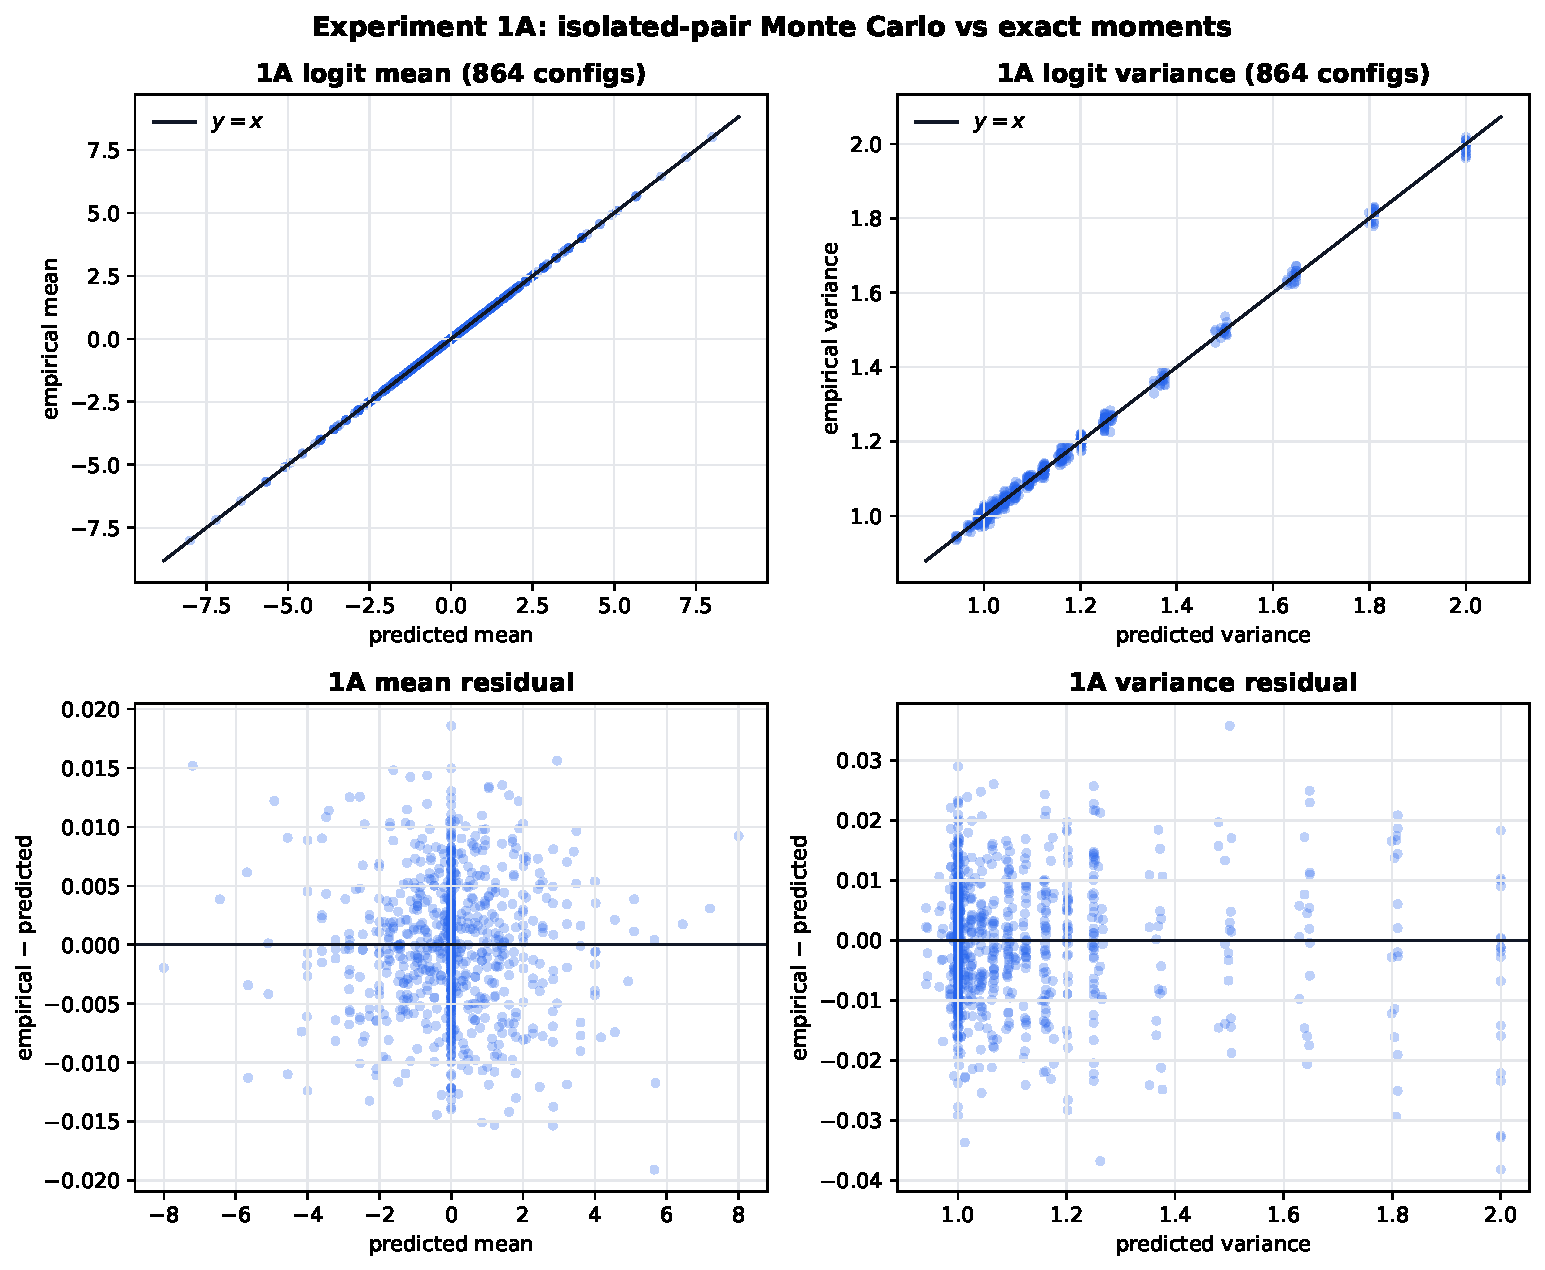
\includegraphics[width=0.98\linewidth]{figures/fig_1a_moment_calibration.pdf}
  \caption{Experiment 1A: isolated-pair Monte Carlo moments versus exact theory. Residuals are centered at zero with magnitude $\sim 10^{-2}$, matching the preregistered precision gate.}
  \label{fig:1a-moments}
\end{figure}

\subsection{Auxiliary check highlights}

\begin{itemize}[leftmargin=*]
  \item Common-bias absolute error: $1.76\times 10^{-4}$ (threshold $0.02$).
  \item Baseline KS $p=0.574$, variance ratio $1.009$.
  \item All 20 gradient configurations: identity error $0$; finite-difference relative errors $\sim 10^{-10}$.
  \item Integration check: initializer changed tensors, checkpoint bitwise equal, forward finite.
\end{itemize}

\subsection{Interpretation of 1A}

The implementation faithfully realizes the finite-width theory within Monte Carlo tolerance. \textbf{Downstream atlas interpretation is unblocked.} Any future failure in 1B--Exp2 cannot be attributed to a Lemma~1 coding error without revisiting this gate.

%=============================================================================
\chapter{Experiment 1B: Discovery Atlas}
%============================================================================

\section{Purpose}

1B empirically maps \textbf{initialization-time attention behavior} across the admissible coefficient domain. Unlike 1A's isolated token pairs, 1B runs a full forward pass through a one-block attention head on \textbf{sequences} of length $n=64$ with value projection and (for the backward probe) a single optimization step.

\section{Reference geometry and grid}

\begin{center}
\begin{tabular}{ll}
\toprule
Parameter & Value \\
\midrule
Token dimension $d$ & 64 \\
Head dimension $m$ & 16 \\
Sequence length $n$ & 64 \\
$\log_2 s$ grid & 17 values in $[-2,2]$ \\
$\alpha$ grid & 13 values in $[-1,1]$ \\
$\phi$ grid & 9 values in $[0,\pi/2]$ \\
Unique cells & $1{,}717$ \\
Seeds per cell & 64 paired seeds \\
\bottomrule
\end{tabular}
\end{center}

\section{Measurement strata}

Each cell is evaluated under \textbf{eight} input/mask strata (per $\phi$ slice, aggregated in analysis):
\begin{enumerate}[leftmargin=*]
  \item Synthetic inputs with token correlation $r=0$, $0.25$, $0.5$ (LayerNorm applied).
  \item \textbf{Real activations}: post-LayerNorm tensors from an independently initialized baseline decoder (distribution shift test).
  \item \textbf{Causal} (lower-triangular) vs.\ \textbf{unmasked} (full) attention.
\end{enumerate}

Raw records per full run: $1{,}717\times 64\times 8 = 879{,}104$ rows (matches \texttt{analysis\_summary.json}).

\section{Analysis pipeline}

\begin{enumerate}[leftmargin=*]
  \item Load all \texttt{atlas\_shard\_*.jsonl} shards ($\sim$1.3\,GB JSONL).
  \item Compute pilot floors from independent baseline $(s,\alpha,\gamma)=(1,0,1)$ (Section~\ref{sec:pilot-thresholds}).
  \item Group rows by $(\mathrm{cell\_id},\mathrm{input\_kind},r,\mathrm{mask},d,m,n)$.
  \item For each group and each of seven metrics, compute median and \textbf{cluster bootstrap 95\% CI} with 2{,}000 draws resampling the 64 seeds.
  \item Assign label + $\pm 0.05$ sensitivity labels.
  \item Export \texttt{atlas\_summary.csv} ($13{,}736$ rows) and 72 stratum phase maps. The analyze-script residual scatter is \emph{not} a 1A replication (Section~\ref{sec:1b-moments}).
\end{enumerate}

\section{Pilot thresholds}
\label{sec:pilot-thresholds}

Derived from the independent baseline at $s=1$ (5th percentile across baseline records):
\begin{center}
\begin{tabular}{ll}
\toprule
Floor & Value \\
\midrule
Jacobian operator norm & 0.0556 \\
Update-to-weight (min of $W_q,W_k$) & $9.75\times 10^{-6}$ \\
Attention effective rank & 0.275 \\
\bottomrule
\end{tabular}
\end{center}

Gradient-starved labels are rare when floors are low; only \textbf{one} stratum in the entire atlas was labeled gradient-starved.

%=============================================================================
\chapter{Experiment 1B Results}
%=============================================================================

\section{Global label histogram}

Pooling all $13{,}736$ stratified summaries:

\begin{center}
\begin{tabular}{lrrl}
\toprule
Label & Count & Percent & Qualitative reading \\
\midrule
Diffuse & 5{,}362 & 39.0\% & Near-uniform attention rows \\
Concentrated & 3{,}793 & 27.6\% & Low entropy or high peak mass \\
Screened candidate & 2{,}867 & 20.9\% & Mid-entropy, passes pathology screens \\
Boundary / uncertain & 1{,}241 & 9.0\% & Thresholds not resolved at 95\% \\
Self-locked & 472 & 3.4\% & High diagonal self-attention \\
Gradient-starved & 1 & $<0.01$\% & Jacobian/update below pilot floor \\
\bottomrule
\end{tabular}
\end{center}

\section{Synthetic vs.\ real activations}

\begin{center}
\begin{tabular}{lrrrrrr}
\toprule
Input kind & Diffuse & Concentrated & Screened & Boundary & Self-locked & Grad-starved \\
\midrule
Synthetic & 4{,}115 & 2{,}811 & 2{,}115 & 960 & 300 & 1 \\
Real activation & 1{,}247 & 982 & 752 & 281 & 172 & 0 \\
\bottomrule
\end{tabular}
\end{center}

Screened fraction: \textbf{24.3\%} synthetic vs.\ \textbf{21.5\%} real (similar order of magnitude; real activations slightly shift mass toward concentrated/self-locked regions).

\section{Reference stratum deep dive}

We highlight \textbf{synthetic, unmasked, $r=0.25$, $\phi=0$}---the canonical ``paper slice'' with $221$ coefficient points (one per admissible $(s,\alpha)$ at this $\phi$).

\begin{center}
\begin{tabular}{lrrrrr}
\toprule
Label & $n$ & Mean $\Hnorm$ & Mean max mass & Mean self-mass & Role \\
\midrule
Diffuse & 99 & 0.990 & 0.028 & 0.017 & High-entropy plateau \\
Screened candidate & 40 & 0.829 & 0.141 & 0.038 & Candidate band \\
Concentrated & 60 & 0.186 & 0.761 & 0.076 & Peaked attention \\
Self-locked & 8 & 0.022 & 0.980 & 0.971 & Diagonal collapse \\
Boundary & 14 & 0.613 & 0.301 & 0.044 & Uncertain \\
\bottomrule
\end{tabular}
\end{center}

At $\phi=\pi/4$ on the same stratum ($n=187$ cells), counts are similar (85 diffuse, 33 screened, 53 concentrated, 3 self-locked), indicating $\phi$ rotates mass between orthogonal/independent components without collapsing the map.

\section{Logit moments inside the 1B forward pass}
\label{sec:1b-moments}

1A tests pairwise moments with many i.i.d.\ draws of $(W_q,W_k)$. 1B stores a \emph{different} diagnostic: for each seed it compares one realized $n\times n$ logit matrix to the closed-form gram formulae. These quantities are not interchangeable.

\paragraph{What is stored.}
Empirical \texttt{logit\_mean} / \texttt{logit\_variance} are the sample mean and sample variance of the realized masked logits $\{\ell_{ij}\}$. Predicted \texttt{predicted\_logit\_mean} is the average of the pairwise conditional means $\mathbb{E}[\ell_{ij}\mid x]$. Predicted \texttt{predicted\_logit\_variance} is the average of the pairwise \emph{conditional} variances $\mathrm{Var}(\ell_{ij}\mid x)$, \textbf{not} the across-pair variance of the map. By the law of total variance,
\[
\mathrm{Var}_{ij}(\ell_{ij})
\;=\;
\mathbb{E}_{ij}\!\bigl[\mathrm{Var}(\ell_{ij}\mid x)\bigr]
\;+\;
\mathrm{Var}_{ij}\!\bigl(\mathbb{E}[\ell_{ij}\mid x]\bigr).
\]
The second term is large whenever $\alpha s^2$ is large (token Gram heterogeneity). Plotting empirical across-pair variance minus mean pairwise conditional variance therefore \emph{must} show structured bands at discrete $s$ values. That is an estimand mismatch, not a 1A failure.

\paragraph{The retracted statistic.}
The previous draft quoted mean residuals $-0.0048\pm 0.0484$ and $+0.0003\pm 0.0013$ as ``excellent agreement.'' Those numbers used only the first $20{,}000$ raw rows (cell ids $0$--$39$, the smallest-scale cells). The analyze-script figure itself was drawn on all $879{,}104$ records. The two do not match, and the global mean residual can cancel opposite stratum biases (e.g.\ $r=0$ vs.\ $r=0.5$).

\paragraph{Full-data calibration (this report).}
On all $879{,}104$ single-draw records, OLS of empirical vs.\ predicted is:

\begin{center}
\begin{tabular}{lrrrrr}
\toprule
Estimand & $a$ & $b$ & $R^2$ & RMSE & Median rel.\ err. \\
\midrule
Mean (raw records) & $0.004$ & $1.001$ & $0.788$ & $1.77$ & $4.7\%$ \\
Mean (seed-averaged, $13{,}736$ strata) & $0.004$ & $1.001$ & $0.996$ & $0.21$ & $0.64\%$ \\
Variance, pairwise formula (raw) & $0.14$ & $1.026$ & $0.920$ & $20.5$ & $17\%$ \\
Variance, pairwise (seed-averaged) & $0.13$ & $1.027$ & $0.949$ & $16.1$ & $16\%$ \\
Variance, total-variance correction (raw) & $-0.06$ & $0.975$ & $0.936$ & $18.3$ & $14\%$ \\
Variance, total-variance (seed-averaged) & $-0.07$ & $0.975$ & $0.965$ & $13.3$ & $8.0\%$ \\
\bottomrule
\end{tabular}
\end{center}

Mean prediction is calibrated ($b\approx 1$). Single-draw residuals are wide ($\mathrm{RMSE}=1.77$); averaging $64$ seeds recovers $R^2=0.996$. That supports the mean formula at sequence scale after Monte Carlo averaging, not per-record precision.

Variance is \textbf{not} ``excellent agreement.'' The pairwise residual mean on the full file is $+0.96\pm 20.4$, not $+0.0003$. Discrete islands in the residual plot coincide with the $17$ values of $s$. Stratified pairwise variance residuals (raw records):

\begin{center}
\begin{tabular}{lrrr}
\toprule
Stratum & Mean residual & RMSE & OLS slope \\
\midrule
Synthetic inputs & $-0.55$ & $20.4$ & $0.98$ \\
Real activations & $+5.46$ & $20.7$ & $1.18$ \\
Unmasked & $+0.27$ & $18.8$ & $1.00$ \\
Causal & $+1.64$ & $22.0$ & $1.05$ \\
$r=0$ & $+5.37$ & $20.5$ & $1.18$ \\
$r=0.25$ & $+0.96$ & $15.3$ & $1.03$ \\
$r=0.5$ & $-7.97$ & $24.3$ & $0.75$ \\
\bottomrule
\end{tabular}
\end{center}

Positive and negative stratum biases cancel in the pooled mean. Adding an off-diagonal Gram estimate of $\mathrm{Var}_{ij}(\mathbb{E}[\ell_{ij}\mid x])$ improves $R^2$ and centers residuals by $s$, but heteroscedasticity remains (spread grows with $s$). The 1A formula is still the right pairwise theory; the 1B stored variance is a different functional of the sequence map.

\begin{figure}[H]
  \centering
  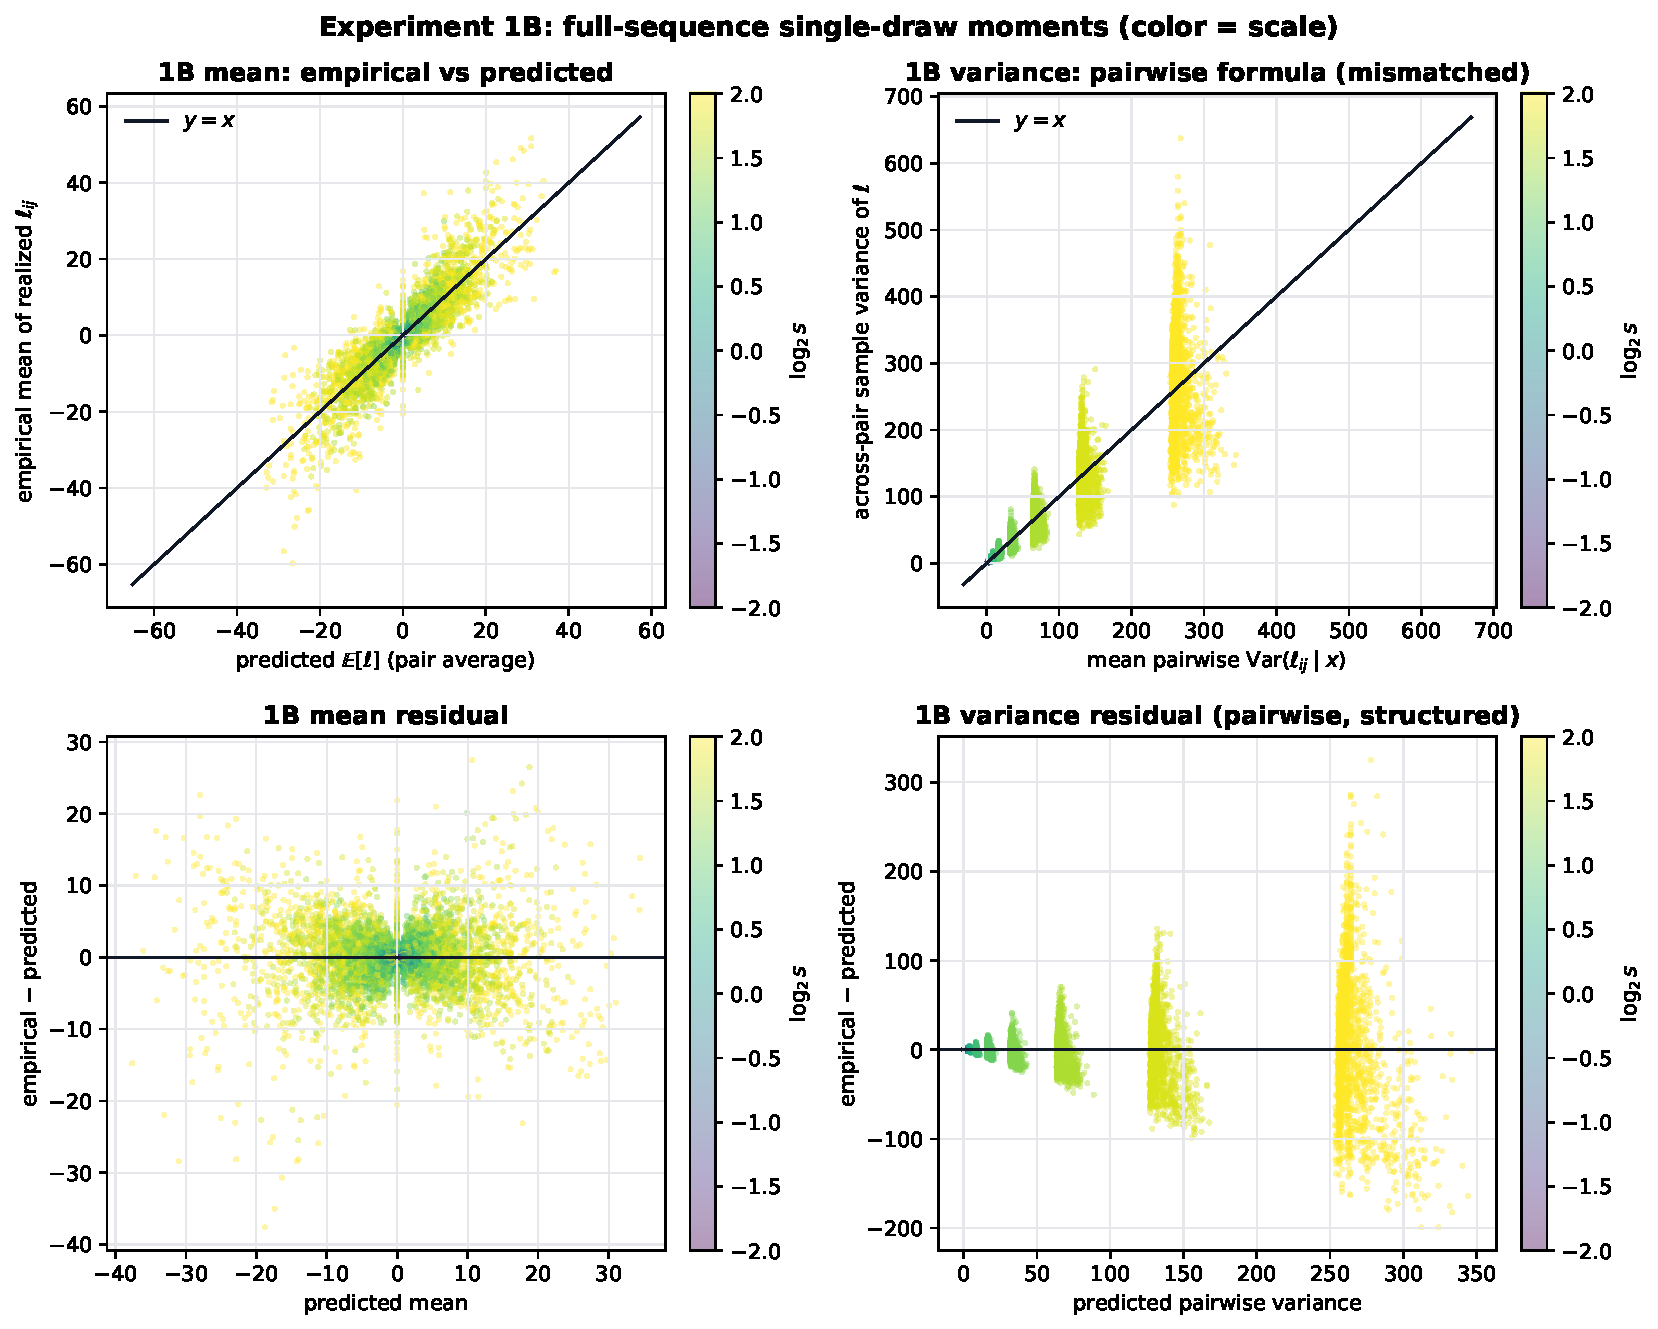
\includegraphics[width=0.98\linewidth]{figures/fig_1b_moment_naive.pdf}
  \caption{1B single-draw diagnostics. Left: mean is approximately unbiased with heteroscedastic scatter. Right: empirical across-pair variance vs.\ mean pairwise conditional variance---mismatched estimands, discrete $s$-bands, large residuals. Color is $\log_2 s$.}
  \label{fig:1b-naive}
\end{figure}

\begin{figure}[H]
  \centering
  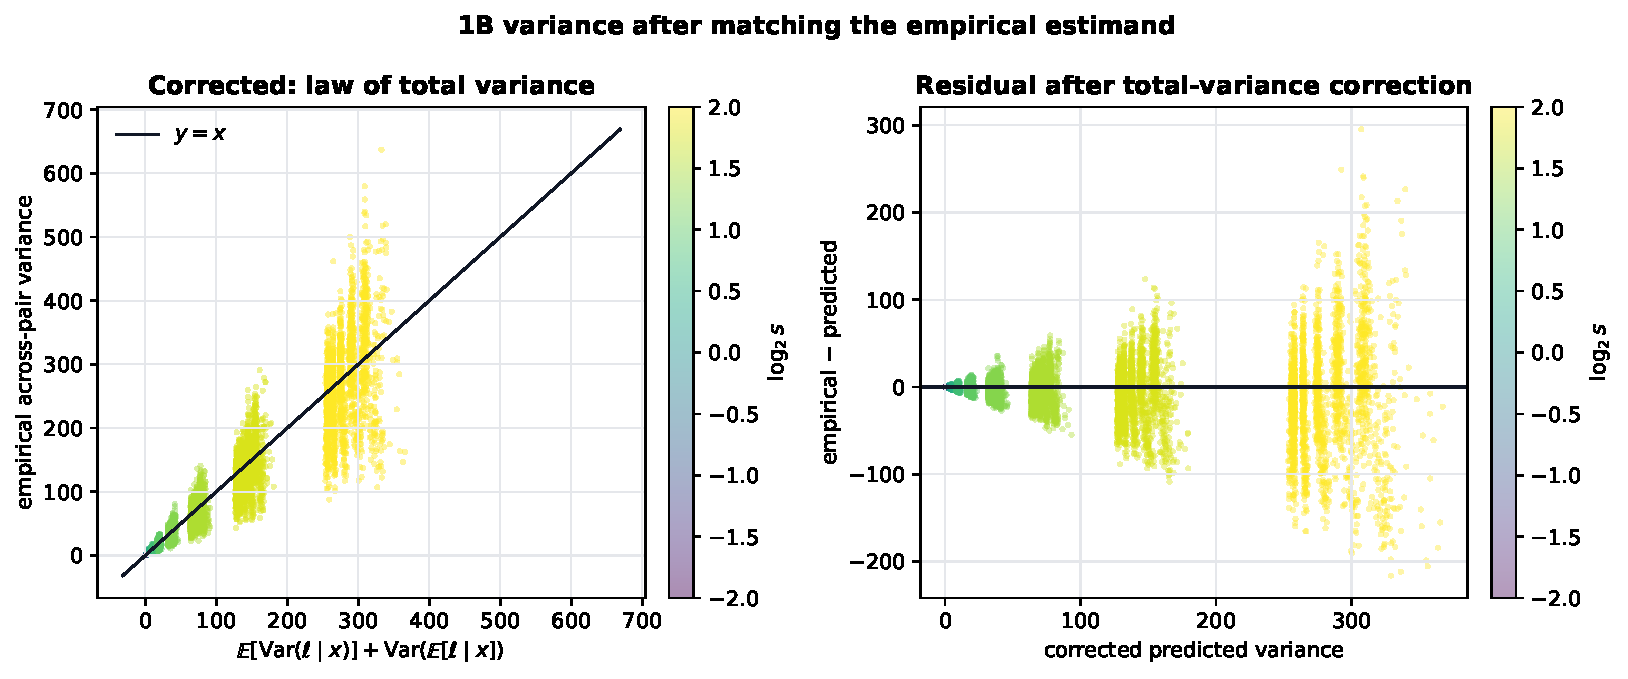
\includegraphics[width=0.98\linewidth]{figures/fig_1b_variance_corrected.pdf}
  \caption{Same empirical variance after adding $\mathrm{Var}_{ij}(\mathbb{E}[\ell_{ij}\mid x])$. Residuals are closer to centered by scale; remaining error is heteroscedastic single-draw noise, not 1A-style $10^{-2}$ Monte Carlo error.}
  \label{fig:1b-corrected}
\end{figure}

\begin{figure}[H]
  \centering
  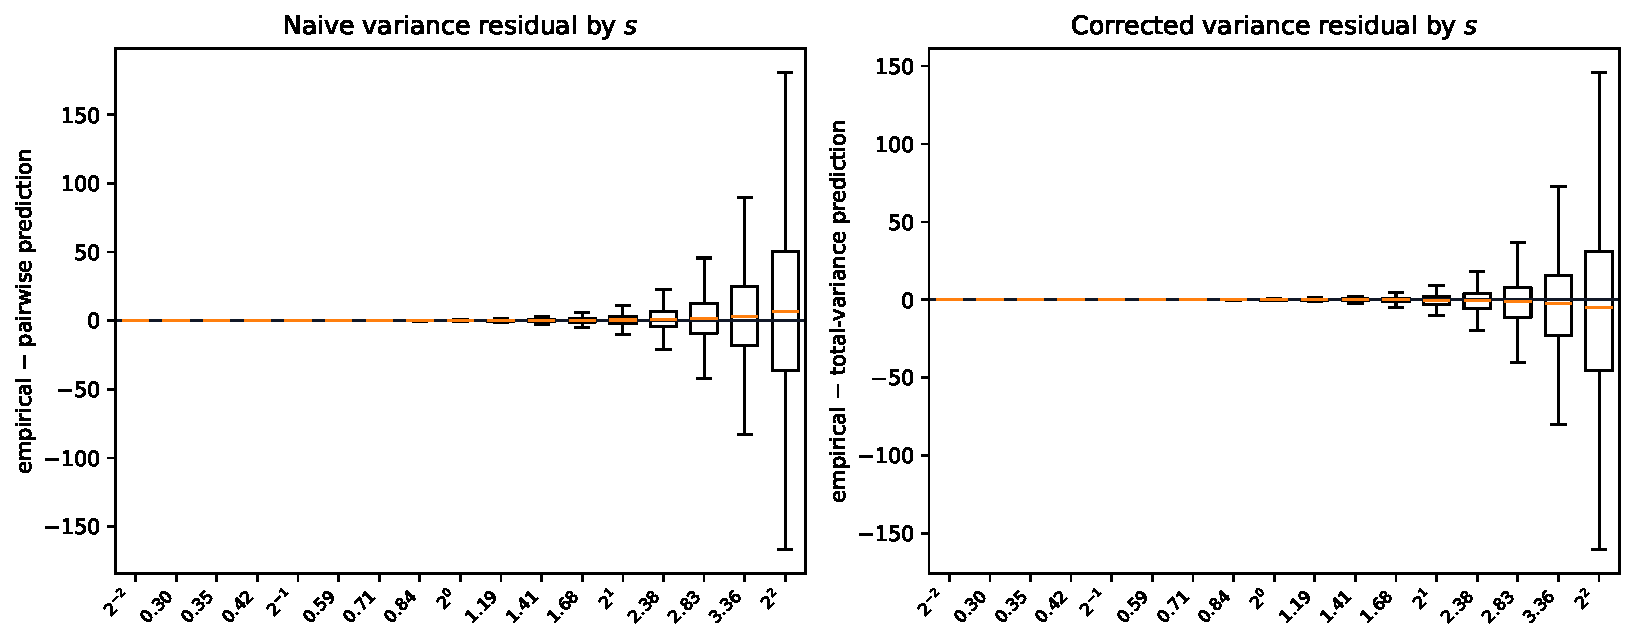
\includegraphics[width=0.98\linewidth]{figures/fig_1b_variance_by_scale.pdf}
  \caption{Variance residuals boxed by $s$. Naive pairwise residuals fan out and shift with scale; the total-variance correction recenters medians. Whiskers at $s=4$ still span $\mathcal{O}(10^2)$.}
  \label{fig:1b-scale}
\end{figure}

\textbf{Conclusion for this section:} 1A remains the confirmatory moment test. 1B means track the theory after seed averaging. 1B variances require matching the across-pair estimand and stratified reporting; they do not license a claim of excellent per-record sequence-scale variance agreement.

\section{Phase-map visualization}

Figure~\ref{fig:regions} follows the reference style used in information-theory phase diagrams: hatched region legend, dashed operational contours, and red-edged dots on the measured $(\log_2 s,\alpha)$ grid. Region~C (screened candidate) is drawn as a \textbf{narrow} horizontal band to avoid overstating its spatial extent.

\begin{figure}[H]
  \centering
  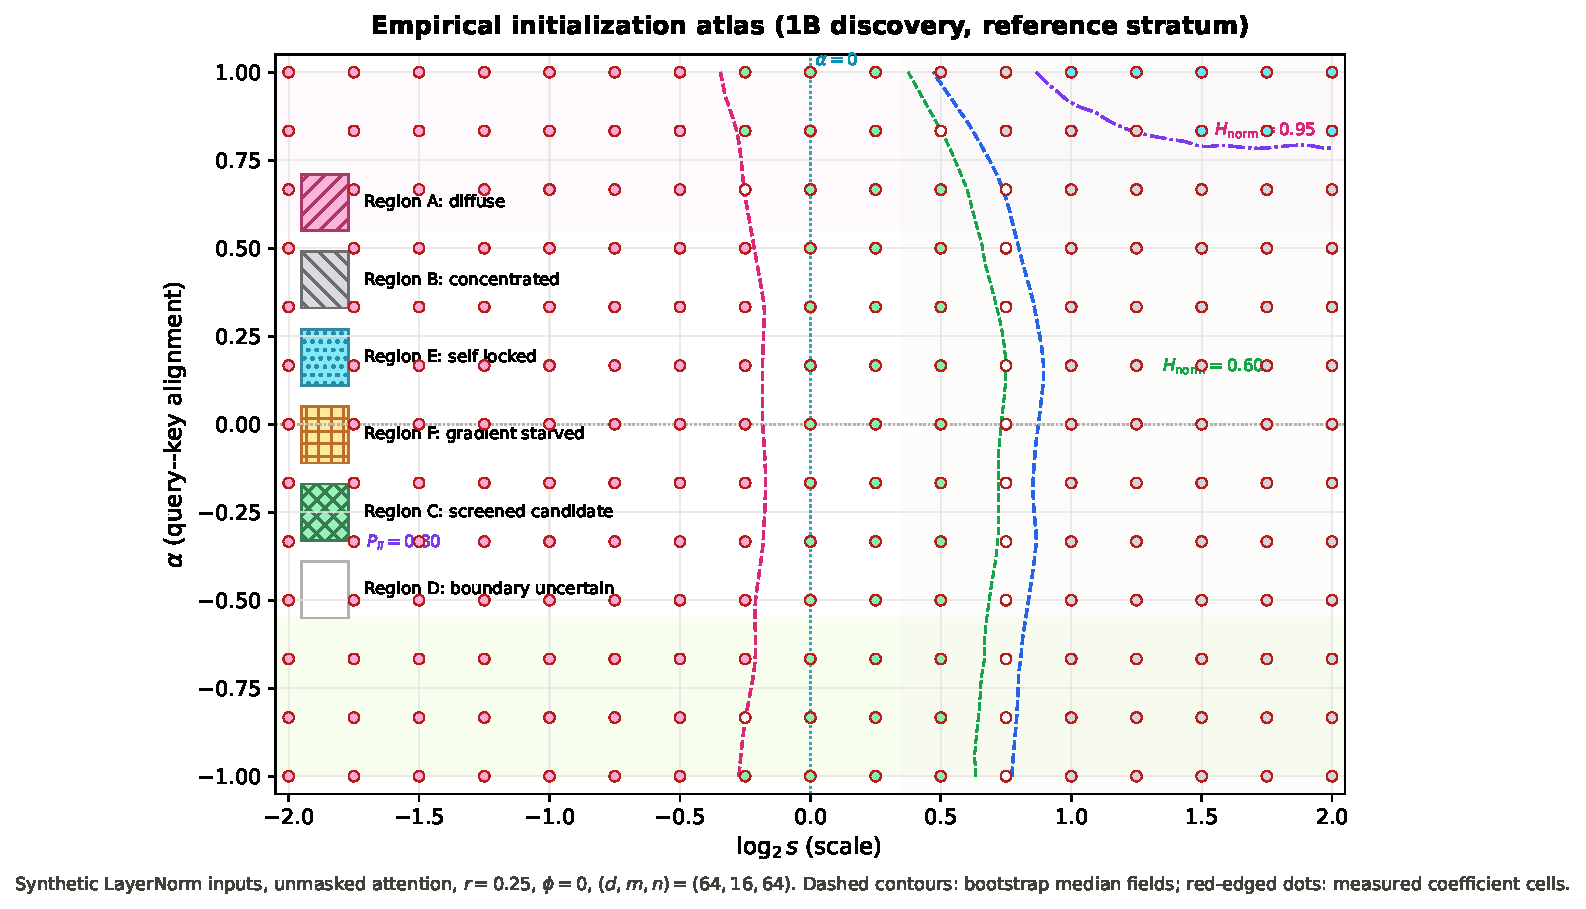
\includegraphics[width=0.98\linewidth]{figures/fig_atlas_regions.pdf}
  \caption{Region-style empirical atlas for the reference stratum. Dashed curves trace interpolated median $H_{\mathrm{norm}}$ and self-mass fields; colored dots are measured cells with preregistered labels.}
  \label{fig:regions}
\end{figure}

Figure~\ref{fig:surface} shows the same data as a smooth surface (analogous to a 3D capacity/entropy landscape).

\begin{figure}[H]
  \centering
  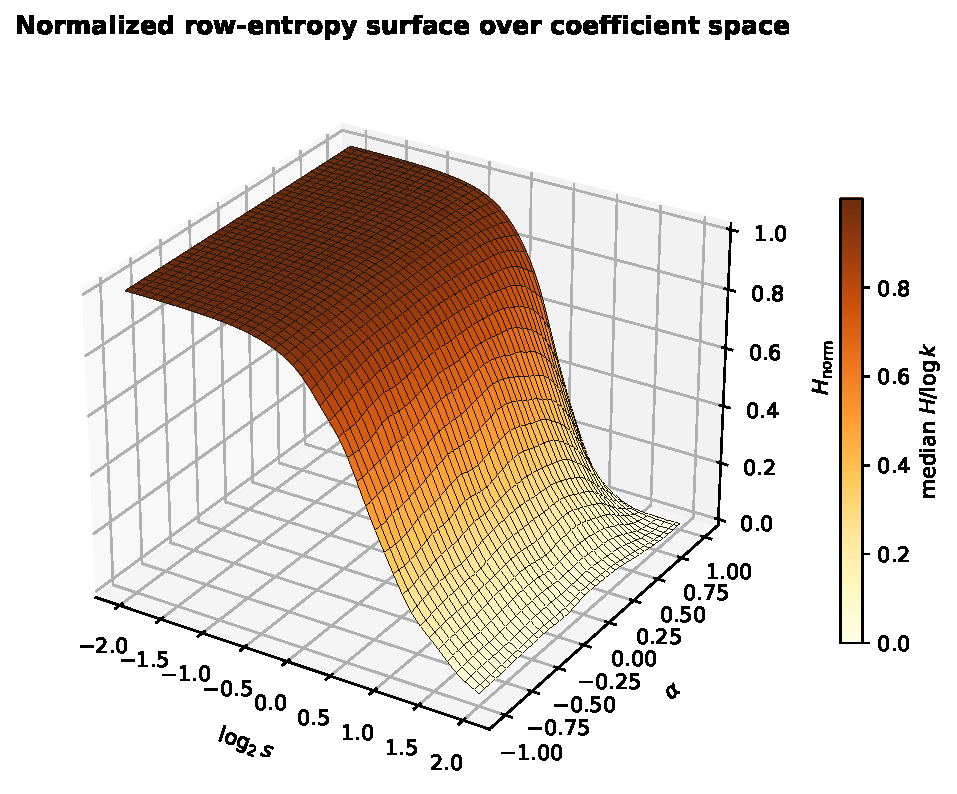
\includegraphics[width=0.88\linewidth]{figures/fig_entropy_surface_3d.pdf}
  \caption{Interpolated normalized row-entropy surface over $(\log_2 s,\alpha)$.}
  \label{fig:surface}
\end{figure}

Figure~\ref{fig:mosaic} gives the discrete nearest-cell label mosaic.

\begin{figure}[H]
  \centering
  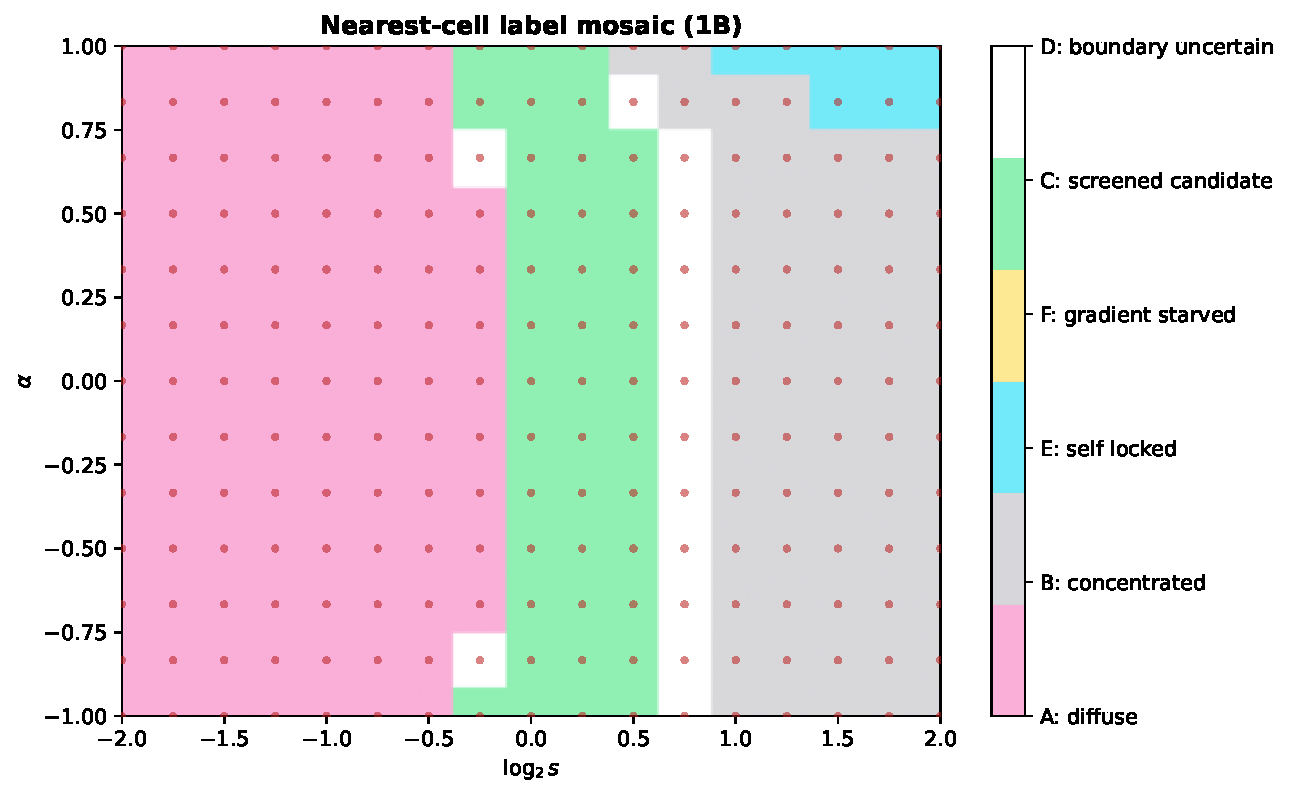
\includegraphics[width=0.92\linewidth]{figures/fig_atlas_label_mosaic.pdf}
  \caption{Nearest-measured-cell label assignment on the coefficient grid.}
  \label{fig:mosaic}
\end{figure}

Legacy scatter plot (analysis script default):

\begin{figure}[H]
  \centering
  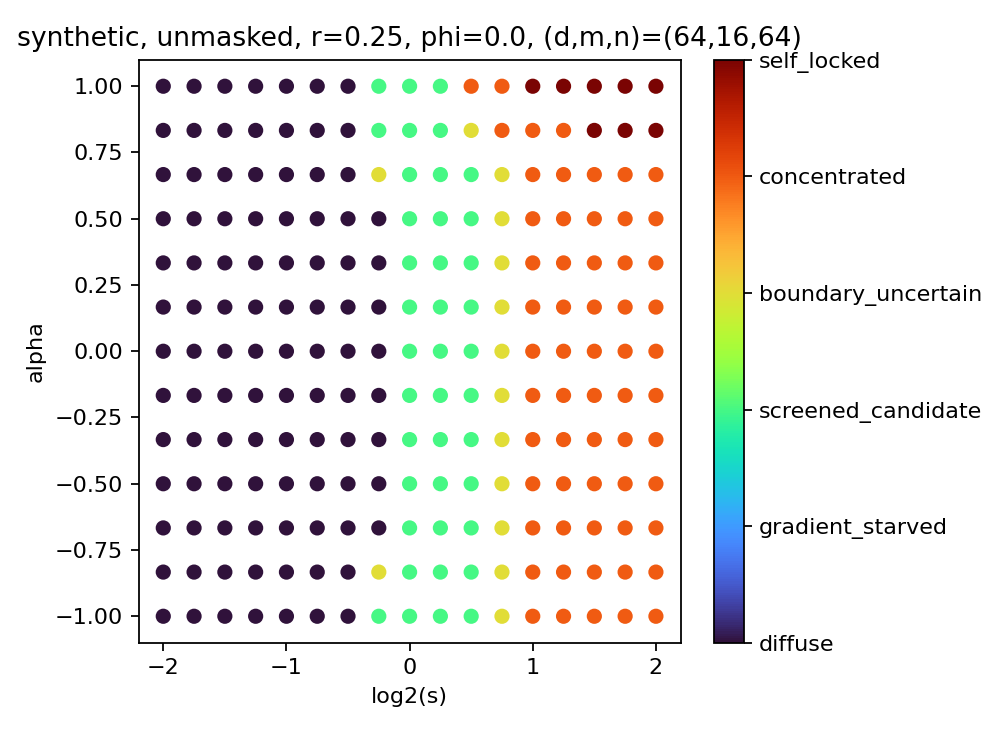
\includegraphics[width=0.78\linewidth]{../../code/exp1b/data/full/figures/atlas_d64_m16_n64_synthetic_unmasked_r0p25_phi0.000000.png}
  \caption{Original turbo-colormap scatter from \texttt{exp1b/run.py} analyze.}
  \label{fig:atlas-ref}
\end{figure}

Additional 71 figures (varying $\phi$, mask, $r$, and real activations) are in \texttt{code/exp1b/data/full/figures/}.

\section{Label stability under threshold perturbation}

Comparing primary labels to $\pm 0.05$ probability/entropy shifts:
\begin{itemize}[leftmargin=*]
  \item $1{,}294$ strata ($9.4\%$) change label under $-0.05$ shift.
  \item $6{,}721$ strata ($48.9\%$) change under $+0.05$ shift.
\end{itemize}

Nearly half the atlas lies near label \textbf{boundaries} under generous threshold perturbation. This is expected: softmax metrics transition continuously. Stage~1C adaptive refinement was run to probe these boundaries (next chapter).

%=============================================================================
\chapter{Experiment 1C: Adaptive Refinement and Transfer}
%=============================================================================

\section{Purpose}

1C fits a probabilistic surrogate on 1B discovery labels, holds out $20\%$ of coefficient cells, proposes $120$ uncertain / theory-disagreement points, and remeasures them at
\[
(d,m,n)\in\{(64,16,64),\ (128,16,128)\}
\]
with $64$ seeds and the same eight input/mask strata as 1B. The freeze rule then requires a coefficient $(s,\alpha,\beta,\gamma)$ to be labeled \texttt{screened\_candidate} on \emph{every} replicated stratum before it can enter \texttt{candidate\_portfolio.json}.

\section{Compute that was merged}

Kaggle produced two archives (\texttt{exp1c.tar}, \texttt{exp1cccc.tar}). Incomplete shards $0002$ and $0003$ from the first archive ($5/30$ tasks) were replaced by the completed copies. Effective sharding was $8$ GPU streams covering all $240$ tasks.

\begin{center}
\begin{tabular}{ll}
\toprule
Item & Value \\
\midrule
Adaptive cells & 120 \\
Geometries & 2 \\
Tasks & 240 (all present) \\
Raw rows & $122{,}880$ ($512$ per task) \\
Stratified summaries & $1{,}920$ \\
Bootstrap draws & $2{,}000$ \\
Pilot floors & Jacobian $0.0241$, update $5.94\times 10^{-6}$, rank $0.175$ \\
\bottomrule
\end{tabular}
\end{center}

\section{Surrogate held-out metrics}

The classifier never trains on the held-out $20\%$ of 1B cells. Reported metrics:

\begin{center}
\begin{tabular}{lr}
\toprule
Metric & Value \\
\midrule
Train / test rows & $10{,}984$ / $2{,}752$ \\
Balanced accuracy & $0.987$ \\
Multiclass log-loss & $0.0355$ \\
Expected calibration error & $0.0153$ \\
Boundary error (top-quartile uncertainty) & $0.0349$ \\
\bottomrule
\end{tabular}
\end{center}

The interpolator is well calibrated on 1B labels. It is \textbf{not} itself evidence that those labels are trainable.

\section{Adaptive-cell labels}

\begin{center}
\begin{tabular}{lrrr}
\toprule
Label & All 1C & $(64,16,64)$ & $(128,16,128)$ \\
\midrule
Diffuse & 793 & 266 & 527 \\
Boundary / uncertain & 613 & 314 & 299 \\
Screened candidate & 514 & 380 & 134 \\
Other pathologies & 0 & 0 & 0 \\
\bottomrule
\end{tabular}
\end{center}

The transfer geometry is substantially more diffuse and less often screened. Majority-label agreement across the two geometries is $30/120$ coefficient points.

On the canonical 1B slice (synthetic, unmasked, $r=0.25$, reference geometry) the $120$ adaptive points are $94$ diffuse, $25$ boundary, and $1$ screened: the sampler did what it was asked to do---it spent budget on uncertain cells, not on the high-entropy plateau.

\section{Why the portfolio did not freeze}

\texttt{freeze\_portfolio} groups rows by $(s,\alpha,\beta,\gamma)$ and keeps a point only if \textbf{all} $16$ copies (2 geometries $\times$ 2 masks $\times$ 4 input correlations/kinds) are \texttt{screened\_candidate}.

\begin{center}
\begin{tabular}{lr}
\toprule
Criterion (120 coefficient points) & Count \\
\midrule
Any stratum screened & 117 \\
Majority of strata screened & 5 \\
All 8 reference-geometry strata screened & 0 \\
All 16 replicated strata screened (freeze rule) & 0 \\
\bottomrule
\end{tabular}
\end{center}

\texttt{candidate\_portfolio.json} therefore records \texttt{frozen: false} (``need 8 replicated screened candidates; found 0''). This is a \textbf{replication-strictness} outcome, not a failed measurement. 1D cannot start on a frozen portfolio until the rule is relaxed (e.g.\ reference geometry only, or majority vote) or more cells are measured.

\section{Label sensitivity}

Of $1{,}920$ 1C strata, $534$ ($27.8\%$) change label under a $-0.05$ probability/entropy shift and $1{,}404$ ($73.1\%$) change under $+0.05$. Adaptive cells sit even closer to decision boundaries than the 1B atlas, which is expected.

%=============================================================================
\chapter{Synthesis and Scientific Reading}
%============================================================================

\section{What 1A established}

The finite-width algebraic theory is not merely analytic---it is implemented correctly in floating point with rigorous Monte Carlo and gradient checks. This is a prerequisite most initialization papers skip.

\section{What 1B established}

\begin{enumerate}[leftmargin=*]
  \item The admissible $(s,\alpha,\phi)$ domain admits \textbf{large, structured regions} of distinct initialization phenotypes (diffuse vs.\ concentrated vs.\ screened).
  \item \textbf{Self-locking} is measurable but occupies a minority ($\sim 3.4\%$ of strata).
  \item \textbf{Gradient starvation} at initialization is extremely rare under the pilot floors ($1$ stratum).
  \item Pairwise mean identities carry over to 1B after seed averaging ($R^2=0.996$). Sequence-scale \emph{variance} as stored in 1B is a different estimand and is only approximately calibrated after a total-variance correction (Section~\ref{sec:1b-moments}); it does not re-prove 1A.
  \item Real activations preserve qualitative label proportions but redistribute mass toward concentration relative to synthetic Gaussians.
\end{enumerate}

\section{What 1C established}

\begin{enumerate}[leftmargin=*]
  \item A discovery surrogate can be fit and held out with balanced accuracy $0.987$ and ECE $0.015$.
  \item The $120$ adaptive cells were fully remeasured at two geometries ($122{,}880$ rows).
  \item Screened labels are \textbf{not} stable under mask, correlation, real activations, and width/length transfer jointly: the preregistered freeze intersection is empty.
  \item Transfer to $(128,16,128)$ shifts mass toward diffuse ($527$ vs.\ $266$ at reference).
\end{enumerate}

\section{What is \emph{not} yet established}

\begin{itemize}[leftmargin=*]
  \item A frozen 8-head \texttt{candidate\_portfolio.json} under the current all-stratum rule.
  \item Whether screened candidates \textbf{train better} (Experiment~1D).
  \item Whether a diverse portfolio improves a 32M LM (Experiment~2).
  \item Sign-symmetry unit test on 50 cells (\texttt{sign\_symmetry\_check.json} not present in the full 1B analyze artifact).
\end{itemize}

%=============================================================================
\chapter{Limitations and Provenance}
\label{ch:limitations}
%=============================================================================

\begin{itemize}[leftmargin=*]
  \item \textbf{Single-block probe}: no depth, no residual stream, no full LM in 1B.
  \item \textbf{One backward step}: update ratios are diagnostic, not training trajectories.
  \item \textbf{Bootstrap draws}: 2{,}000 (manifest \texttt{exp1b\_1788602938369\_18144.json}); coarser than preregistered 10{,}000 but sufficient for exploration.
  \item \textbf{CPU/RAM analyze}: $\sim$1.3\,GB JSONL loaded fully into memory.
  \item \textbf{Labels are descriptive}, not causal claims about generalization.
  \item \textbf{1B logit variance is not the 1A estimand}: \texttt{predicted\_logit\_variance} averages pairwise conditional variances; \texttt{logit\_variance} is the across-pair sample variance of one realized map. Pooled mean residuals cancel opposing $r$ and input-kind biases.
  \item \textbf{1C freeze is strict}: a point must be screened on all 16 replicated strata. Zero of 120 points pass; 1D is blocked until the rule is changed or more cells are collected.
  \item \textbf{Git LFS}: raw shards require \texttt{git lfs pull} or manual upload on cloud machines.
\end{itemize}

\textbf{Artifact paths:}
\begin{itemize}[leftmargin=*]
  \item 1A: \texttt{code/exp1a/data/full/gate\_summary.json}, \texttt{moment\_results.json}, \texttt{checks.json}
  \item 1B: \texttt{code/exp1b/data/full/analysis\_summary.json}, \texttt{atlas\_summary.csv}, \texttt{figures/}
  \item 1C: \texttt{code/exp1c/data/full/analysis\_summary.json}, \texttt{atlas\_summary.csv}, \texttt{candidate\_portfolio.json}, \texttt{held\_out\_metrics.json}
\end{itemize}

%=============================================================================
\chapter{Recommended Next Steps}
%=============================================================================

\begin{enumerate}[leftmargin=*]
  \item \textbf{Unblock 1C freeze}: either require screening only on the reference geometry / majority vote, or propose additional cells around the 5 majority-screened coefficients.
  \item \textbf{1D}: once a portfolio is frozen, train one-block decoder on associative recall + TinyStories; test screened vs.\ pathology early-loss gate.
  \item \textbf{Exp2}: 32M LM confirmatory study with frozen treatments.
\end{enumerate}

\appendix
\chapter{Holm--Bonferroni reminder}

Given ordered $p$-values $p_{(1)}\le\dots\le p_{(m)}$, reject hypothesis $i$ if $p_{(i)}\le \alpha/(m-i+1)$. We applied $m=1728$, $\alpha=0.01$ in 1A.

\chapter{Bootstrap procedure in 1B}

For each stratum with seed values $\{x_s\}_{s=1}^{64}$:
\begin{enumerate}[leftmargin=*]
  \item Resample 64 seeds with replacement $B=2000$ times.
  \item Compute median metric per resample.
  \item Report 2.5\% and 97.5\% quantiles as CI endpoints.
\end{enumerate}
Seeds are paired across cells; heads/tokens nested within seed are not separate bootstrap units (cluster bootstrap at seed level).

\end{document}
